\chapter{$\DTCWT$ Single Subband Gains}\label{app:ch6:dtcwt}
This appendix proves that the $\DTCWT$ \emph{gain layer} proposed in
\autoref{ch:freqlearn} maintains the shift invariant properties of the
$\DTCWT$.

Recall that with multirate systems, upsampling by $M$ takes $X(z)$ to
$X(z^M)$ and downsampling by $M$ takes $X(z)$ to $\frac{1}{M}\sum_{k=0}^{M-1} X(W_M^k
z^{1/M})$ where $W_M^k = e^{\frac{j2\pi k}{M}}$. We will drop the $M$ subscript
below unless it is unclear of the sample rate change, simply using $W^k$.


\section{Revisiting the Shift Invariance of the $\DTCWT$}
\begin{figure}[t]
  \centering
  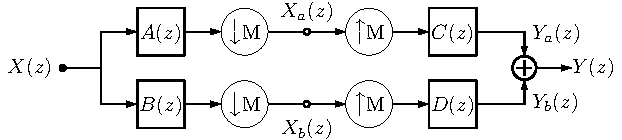
\includegraphics{\imgpath/dtcwt.pdf}
  % \begin{tikzpicture}
    \matrix (m1) [minimum height=4mm, column sep=6mm, align=center]
	{
	%--------------------------------------------------------------------
		\node[coordinate]                  (m00) {};    &
		\node[coordinate]                  (m01) {};          &
		\node[dspsquare]                   (m02) {$A(z)$};          &
		\node[circle,draw,inner sep=1pt]   (m03) {\downsamplertext{M}}; &
		\node[dspnodeopen,dsp/label=above] (m04) {$X_a(z)$};          &
		\node[circle,draw,inner sep=1pt]   (m07) {\upsamplertext{M}}; &
		\node[dspsquare]                   (m08) {$C(z)$};          &
		\node[coordinate]                  (m09) {};          &
		\node[coordinate]                  (m0X) {};          \\
		%--------------------------------------------------------------------
		\node[dspnodefull]                 (m10) {};          &
		\node[coordinate]                  (m11) {};          &
		\node[coordinate]                  (m12) {};    &
		\node[coordinate]                  (m13) {};          &
		\node[coordinate]                  (m14) {};    &
		\node[coordinate]                  (m17) {};          &
		\node[coordinate]                  (m18) {};    &
		\node[dspadder]                    (m19) {};          &
		\node[]     (m1X) {};          \\
		%--------------------------------------------------------------------
		\node[coordinate]                  (m20) {};    &
		\node[coordinate]                  (m21) {};          &
		\node[dspsquare]                   (m22) {$B(z)$};          &
		\node[circle,draw,inner sep=1pt]   (m23) {\downsamplertext{M}}; &
		\node[dspnodeopen,dsp/label=below] (m24) {$X_b(z)$};          &
		\node[circle,draw,inner sep=1pt]   (m27) {\upsamplertext{M}}; &
		\node[dspsquare]                   (m28) {$D(z)$};          &
		\node[coordinate]                  (m29) {};          &
		\node[coordinate]                  (m2X) {};          \\
		%--------------------------------------------------------------------
	};
	\draw[dspline] (m10) -- (m11);
	\draw[dspline] (m11) -- (m01);
	\draw[dspline] (m11) -- (m21);
	\foreach \i in {0,2} {
    	\draw[dspconn] (m\i1) -- (m\i2);
    	\draw[dspconn] (m\i2) -- (m\i3);
    	\draw[dspline] (m\i3) -- (m\i4);
    	\draw[dspconn] (m\i4) -- (m\i7);
    	\draw[dspconn] (m\i7) -- (m\i8);
    	\draw[dspline] (m\i8) -- (m\i9);
	}
  \node[left=0pt of m10] (left) {$X(z)$};
  \node[below=9pt of m24] (bottom) {};
  \draw[dspconn] (m09) -- node[right, yshift=5pt] {$Y_a(z)$} (m19);
  \draw[dspconn] (m29) -- node[right, yshift=-5pt] {$Y_b(z)$} (m19);
  \draw[dspconn] (m19) -- node[right, xshift=5pt] {$Y(z)$} (m1X);
	
\end{tikzpicture}

  \mycaption{Block Diagram of 1-D $\DTCWT$}{Note the top and bottom paths are
  through the wavelet or scaling functions from just level m ($M=2^m$). Figure
  based on Figure~4 in \cite{kingsbury_complex_2001}.}
  \label{fig:ch6:dtcwt_two_tree}
\end{figure}
It is easiest to prove the shift invariance of the gain layer by expanding on
the shift invariance of the $\DTCWT$ proofs done in
\cite{kingsbury_complex_2001}.

Let us consider one subband of the $\DTCWT$. This includes the coefficients from
both tree A and tree B. For simplicity in this analysis we will consider the 1-D
$\DTCWT$ without the channel parameter $c$. 

If we only keep coefficients from a given
subband and set all the others to zero, then we have a reduced tree as shown in
\autoref{fig:ch6:dtcwt_two_tree}. The output $Y(z)$ is:
%
\begin{equation}
  Y(z) = \frac{1}{M} \sum_{k=0}^{M-1}X(W^k z) \left[A(W^k z)C(z) + B(W^k z)D(z)\right]
  \label{eq:ch6:aliasing}
\end{equation}
%
where the aliasing terms are formed from the addition of the rotated z
transforms, i.e.\ when $k \neq 0$.

\begin{theorem} \label{thm:ch6:shiftinv}
  The aliasing terms for \eqref{eq:ch6:aliasing} cancel out if the impulse
  responses of $B$ and $D$ are Hilbert transforms of the impulse responses of
  $A$ and $C$ respectively, and the system in \autoref{fig:ch6:dtcwt_two_tree}
  is nearly shift invariant.
\end{theorem}

\begin{proof}
  See section 4 of \cite{kingsbury_complex_2001} for the full proof of
  this, and section 7 for the bounds on what `nearly' shift invariant means. 
\end{proof}

Consider the complex filters defined as:
\begin{align}
  P(z) &= \frac{1}{2}\left(A(z) + jB(z)\right) \\
  Q(z) &= \frac{1}{2}\left(C(z) - jD(z)\right)
\end{align}
and define $P^*(z) = \sum_{n} p^{*}[n] z^{-n}$ as the $Z$-transform of $p$
after taking the complex conjugate of the filter taps. 

From this, we can rewrite the filters $A, B, C$ and $D$ as:
\begin{align}
  A(z) &= P(z) + P^*(z) \\
  B(z) &= -j(P(z) - P^*(z)) \\
  C(z) &= Q(z) + Q^*(z) \\
  D(z) &= j(Q(z) - Q^*(z))
\end{align}

Substituting these into \eqref{eq:ch6:aliasing} gives:
\begin{equation}
  A(W^k z)C(z) + B(W^k z)D(z) = 2P(W^kz)Q(z) + 2P^*(W^kz)Q^*(z) \label{eq:ch6:complex_filts}
\end{equation}
Using \eqref{eq:ch6:complex_filts}, Kingsbury show that if $B$ is the Hilbert pair
of $A$ then $P$ has support only on the right hand side of the frequency plane.
Similarly if $D$ is the Hilbert pair of $C$ then $Q$ also has support only on
the right hand side of the frequency plane. If $P$ and $Q$ are single side band,
then so are $P^*$ and $Q^*$, but they now have support only on the left hand
side of the frequency plane. 

Given these properties, the shifted versions of $P(W^k z)$ have negligible overlap
with $Q(z)$ except for $k=0$ (the wanted term) and $k=\pm 1$ where the
transition bands overlap. Similarly $P^*(W^k z)$ only overlaps with $Q^*(z)$ 
when $k=0$ and a small amount for $k = \pm 1$. \cite{kingsbury_complex_2001}
quantify the amount of transition band overlap and show it is negligible.

This means $A(W^k z)C(z) + B(W^k z)D(z) = 0$ when $k\neq 0$ and 
\eqref{eq:ch6:aliasing} reduces to:
\begin{equation}
  Y(z) =  \frac{1}{M} X(z)\left[ A(z)C(z) + B(z)D(z) \right]
  \label{eq:ch6:aliasing_cancel} 
\end{equation}

\section{Gains in the Subbands}
\begin{figure}[t]
  \centering
  % \begin{tikzpicture}
    \matrix (m1) [row sep=5mm, column sep=6mm,align=center,anchor=center]
	{
	%--------------------------------------------------------------------
		\node[coordinate]                  (m00) {};    &
		\node[coordinate]                  (m01) {};          &
		\node[dspsquare]                   (m02) {$A(z)$};          &
		\node[circle,draw,inner sep=1pt]   (m03) {\downsamplertext{M}}; &
		\node[dspnodeopen,dsp/label=above] (m04) {$U_a(z)$};          &
    \node[rectangle,draw,inner sep=2pt](m05) {$G_{aa}(z)$}; &
		\node[dspnodeopen,dsp/label=above] (m06) {$V_a(z)$};          &
		\node[circle,draw,inner sep=1pt]   (m07) {\upsamplertext{M}}; &
		\node[dspsquare]                   (m08) {$C(z)$};          &
		\node[coordinate]                  (m09) {};          &
		\node[coordinate]                  (m0X) {};          \\
		%--------------------------------------------------------------------
      \node[dspnodefull]                 (m10) {};          &
		\node[coordinate]                  (m11) {};          &
		\node[coordinate]                  (m12) {};    &
		\node[coordinate]                  (m13) {};          &
		\node[coordinate]                  (m14) {};    &
		\node[coordinate]                  (m15) {};          &
		\node[coordinate]                  (m16) {};    &
		\node[coordinate]                  (m17) {};          &
		\node[coordinate]                  (m18) {};    &
		\node[dspadder]                    (m19) {};          &
    \node[]                            (m1X) {$Y(z)$};          \\
		%--------------------------------------------------------------------
		\node[coordinate]                  (m20) {};    &
		\node[coordinate]                  (m21) {};          &
		\node[dspsquare]                   (m22) {$B(z)$};          &
		\node[circle,draw,inner sep=1pt]   (m23) {\downsamplertext{M}}; &
		\node[dspnodeopen,dsp/label=below] (m24) {$U_b(z)$};          &
      \node[rectangle,draw,inner sep=2pt](m25) {$G_{bb}(z)$}; &
		\node[dspnodeopen,dsp/label=below] (m26) {$V_b(z)$};          &
		\node[circle,draw,inner sep=1pt]   (m27) {\upsamplertext{M}}; &
		\node[dspsquare]                   (m28) {$D(z)$};          &
		\node[coordinate]                  (m29) {};          &
		\node[coordinate]                  (m2X) {};          \\
		%--------------------------------------------------------------------
  };
	\draw[dspline] (m10) -- (m11);
	\draw[dspline] (m11) -- (m01);
	\draw[dspline] (m11) -- (m21);
	\foreach \i in {0,2} {
    	\draw[dspconn] (m\i1) -- (m\i2);
    	\draw[dspconn] (m\i2) -- (m\i3);
    	\draw[dspline] (m\i3) -- (m\i4);
    	\draw[dspconn] (m\i4) -- (m\i5);
    	\draw[dspline] (m\i5) -- (m\i6);
    	\draw[dspconn] (m\i6) -- (m\i7);
    	\draw[dspconn] (m\i7) -- (m\i8);
    	\draw[dspline] (m\i8) -- (m\i9);
	}
	%\draw[dspflow] (m04) --  (m06);
	%\draw[dspflow] (m24) -- (m26);
  \draw[dspconn] (m24) -- node[draw,pos=0.7,inner sep=2pt,fill=white] {$G_{ba}(z)$} (m06);
  \draw[dspconn] (m04) -- node[draw,pos=0.7,inner sep=2pt,fill=white] {$G_{ab}(z)$} (m26);
  \draw[dspconn] (m09) -- node[right] {$Y_a(z)$} (m19);
  \draw[dspconn] (m29) -- node[right] {$Y_b(z)$} (m19);
	\draw[dspconn] (m19) -- (m1X);
  \node[left=0pt of m10] (left) {$X(z)$};
  \node[below=10pt of m24] (bottom) {};
	
\end{tikzpicture}

  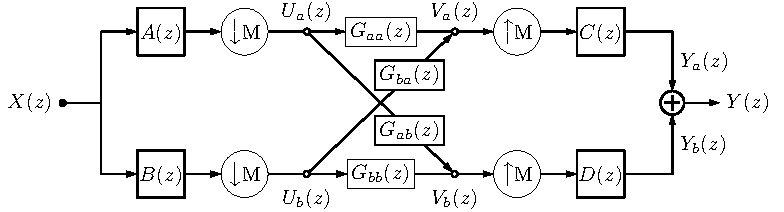
\includegraphics{\imgpath/dtcwt2.pdf}
  \mycaption{Block Diagram of 1-D $\DTCWT$ with subband gains}{}
  \label{fig:ch6:dtcwt_two_tree_gain}
\end{figure}

\autoref{fig:ch6:dtcwt_two_tree_gain} shows a block diagram of the extension of 
the above to general gains. This is a two port network with four individual
transfer functions. Let the transfer fucntion from $U_i$ to $V_j$
be $G_{ij}$ for $i, j \in \{a, b\}$. Then $V_a$ and $V_b$ are:
\begin{eqnarray}
  V_a(z) &=& U_a(z)G_{aa}(z) + U_b(z)G_{ba}(z) \\
         &=& \frac{1}{M} \sum_k X(W^{k} z^{1/M}) \left[A(W^k z^{1/M})G_{aa}(z) +
             B(W^k z^{1/M}) G_{ba}(z) \right] \\
  V_b(z) &=& U_a(z)G_{ab}(z) + U_b(z)G_{bb}(z) \\
         &=& \frac{1}{M} \sum_k X(W^{k} z^{1/M}) \left[A(W^k z^{1/M})G_{ab}(z) +
             B(W^k z^{1/M}) G_{bb}(z) \right] 
\end{eqnarray}
%
Further, $Y_a$ and $Y_b$ are:
\begin{eqnarray}
  Y_a(z) &=& C(z)V_a(z^M) \\
  Y_b(z) &=& D(z)V_b(z^M)
\end{eqnarray}
%
Then the output is:
\begin{alignat}{2}
    Y(z) &= Y_{a}(z) + Y_{b}(z) \\
         &= \frac{1}{M} \sum_{k=0}^{M-1} X(W^k z) & \left[  A(W^kz)C(z)G_{aa}(z^M) + B(W^kz)D(z)G_{bb}(z) + \right. \nonumber \\
         &                                        & \left. \hphantom{[}  B(W^kz)C(z)G_{ba}(z^M) + A(W^kz)D(z)G_{ba}(z) \right] 
    \label{eq:ch6:transfer}
\end{alignat}
% \begin{equation}
  % \begin{split}
  % % \begin{multline}
    % Y(z) &= Y_{a}(z) + Y_{b}(z) \\
    % &= \frac{1}{M} \sum_{k=0}^{M-1} X(W^k z)
    % & \left[  A(W^kz)C(z)G_{aa}(z^M) + B(W^kz)D(z)G_{bb}(z) + \right. \\
    % & \left. \hphantom{[}  B(W^kz)C(z)G_{ba}(z^M) + A(W^kz)D(z)G_{ba}(z) \right] 
    % \label{eq:ch6:transfer}
  % % \end{multline}
  % \end{split}
% \end{equation}

\begin{theorem}\label{thm:ch6:shiftinvgain}
  If we let $G_{aa}(z) = G_{bb}(z) = G_r(z)$ and $G_{ab}(z) = -G_{ba}(z) = G_i(z)$
  then the end to end transfer function is shift invariant. 
\end{theorem}
\begin{proof}
  Using the above substitutions, the terms in the square brackets of
  \eqref{eq:ch6:transfer} become:
  \begin{equation}\label{eq:ch6:realimag}
    G_r(z^M)\left[A(W^kz)C(z) + B(W^kz)D(z)\right] + G_i(z^M)\left[A(W^kz)D(z) - B(W^kz)C(z)\right]
  \end{equation}
  \autoref{thm:ch6:shiftinv} already showed that the $G_r$ terms are shift
  invariant and reduce to $A(z)C(z) + B(z)D(z)$. To prove the same for the $G_i$
  terms, we follow the same procedure. Using our definitions of $A, B, C, D$
  from \autoref{thm:ch6:shiftinv} we note that:
  %
  \begin{eqnarray}
    A(W^kz)D(z) - B(W^kz)C(z) &=& j\left[P(W^kz) + P^*(W^kz)\right]\left[Q(z) -Q^*(z)\right] +\\
                              &&j\left[P(W^kz) -P^*(W^kz)\right]\left[Q(z) + Q^*(z)\right] \\
                              &=& 2j\left[P(W^kz)Q(z) - P^*(W^kz)Q^*(z)\right]
  \end{eqnarray}
  We note that the difference
  between the $G_r$ and $G_i$ terms is just in the sign of the negative
  frequency parts, i.e. $AD - BC$ is the Hilbert pair of $AC+BD$. To prove shift
  invariance for the $G_r$ terms in \autoref{thm:ch6:shiftinv}, we ensured that
  $P(W^kz)Q(z) \approx 0$ and $P^*(W^kz)Q^*(z) \approx 0$ for $k\neq 0$. We can
  use this again here to prove the shift invariance of the $G_i$ terms in
  \eqref{eq:ch6:realimag}. This completes our proof.
\end{proof}

Using \autoref{thm:ch6:shiftinvgain}, the output is now
\begin{align}
  Y(z) &= \frac{2}{M} X(z) \left[G_r(z^{M}) \left(AC + BD\right)
  + G_i(z^{M}) \left(AD - BC\right) \right] \\
  &= \frac{2}{M}X(z)\left[G_r(z^{M}) \left(PQ + P^*Q^*\right)
  + G_i(z^{M}) \left(PQ - P^*Q^*\right) \right]  \label{eq:ch6:end2end}
\end{align}
where we have dropped the $z$ terms on $A, B, C, D, P, Q$ for brevity.

\begin{theorem}\label{thm:ch6:complex_multiply}
  If we treat the two subband coefficients as a complex value $U(z) = U_a(z) +
  jU_b(z)$ then doing a complex multiply by a gain $G(z) = G_r(z) + jG_i(z)$
  maintains shift invariance.
\end{theorem}
\begin{proof}
  This follows from the conditions in \autoref{thm:ch6:shiftinvgain}. There we
  saw that we maintained shift invariance if 
  $G_{aa}(z) = G_{bb}(z) = G_r(z)$ and $G_{ab}(z) = -G_{ba}(z) = G_i(z)$. 
  If we consider $V$ as a complex signal given by $V(z) = V_a(z) + jV_b(z)$, we
  can see from \autoref{fig:ch6:dtcwt_two_tree_gain} that the real and imaginary
  parts of $V$ are:
  \begin{align}
    V_a(z) &= G_r(z) U_a(z) - G_i(z) U_b(z) \\
    V_b(z) &= G_r(z) U_b(z) + G_i(z) U_a(z) 
  \end{align}
  which follows the form of a complex multiply.
\end{proof}

Now we know can assume that our $\DTCWT$ is well designed and extracts frequency
bands at local areas, then our complex filter $G(z)=G_r(z) + jG_i(z)$ allows us
to modify these passbands (e.g.\ by simply scaling if $G(z) = C$, or by more
complex functions.
\autoref{thm:ch6:complex_multiply} and \eqref{eq:ch6:end2end} give us an intuiton for the real and
imaginary parts of a complex gain $G$. The real part $G_r$ affects how much of
the bandpass gain $PQ + P^*Q^*$ propagetes through, and the imaginary part $G_i$
affects how much its Hilbert pair $PQ-P^*Q^*$ propagates.
